% ZhCvGo15.tex      pdflatex ZhCvGo15

% Diffuse globally, compute locally: a cyclist tale
% Tingnan Zhang, Daniel I. Goldman and Predrag Cvitanovi\'c

                  %%   logical setup, no need to edit %%%%%%%%%%
                  \newif\ifpaper \paperfalse \newif\ifPDF \PDFtrue %%
                  \newif\ifboyscout %%
                  \boyscouttrue %% commented, WWW/drafts %%
%%%% Toggle between draft and public versions
% \boyscoutfalse % public, for hyperlinked pdf

% Predrag                       2015-11-19
% Tingnan                       2015-11-

        \ifboyscout
\documentclass[aps,pre,
                showpacs,
                twocolumn,
                %preprint,      %uncomment for double spacing
                groupedaddress,
                floatfix]{revtex4-1}
        \else
\documentclass[pre,aps,
                twocolumn,
                showpacs,
                superscriptaddress,
                groupedaddress,
                floatfix,
                hyperref]{revtex4-1}
        \fi
%   REVTeX 4 Version 4.1r August 2010
%   Phys. Rev. appearance, change preprint to twocolumn.  Choose pra,
%   prb, prc, prd, pre, prl, prstab for journal Add
%   'draft' option to mark overfull boxes with black boxes Add
%   'showpacs' option to make PACS codes appear Add 'showkeys' option
%   to make keywords appear
% Use the \preprint command to place your local institutional report
% number in the upper righthand corner of the title page in preprint
% mode.  Multiple \preprint commands are allowed.  Use the
% 'preprintnumbers' class option to override journal defaults to
% display numbers if necessary \preprint{}

\input ../inputs/setupSveZha
\input ../inputs/editsDasbuch %% editing comments, DasBuch style
\input ../inputs/def %% do not edit; update from dasbuch/book/inputs/def.tex
\input ../inputs/defsSveZha %% all diffusion project edits: \renewcommand, etc

\begin{document}

\title{Discrete factorization of deterministic diffusion}
\author{Tingnan Zhang}
\author{Daniel I. Goldman}
\author{Predrag Cvitanovi\'c}

\email[]{predrag@gatech.edu}
\homepage[]{ChaosBook.org}
\thanks{NSF DMS-1211827}
\affiliation{School of Physics, Georgia Institute of Technology, Atlanta GA}
%   Group addresses by affiliation; use superscriptaddress for long
%   author lists, or if there are many overlapping affiliations.
% repeat the \author .. \affiliation etc. as needed \email, \thanks,
% \homepage, \altaffiliation all apply to the current
% author. Explanatory text should go in the []'s, actual e-mail
% address or url should go in the {}'s for \email and \homepage.
% Please use the appropriate macro foreach each type of information

% \affiliation command applies to all authors since the last
% \affiliation command. The \affiliation command should follow the
% other information \affiliation can be followed by \email, \homepage,
% \thanks as well.


\date{\today}

\begin{abstract}
  \input abstract
\end{abstract}

% insert suggested PACS numbers in braces on next line
\pacs{
05.10.-a,   %Computational methods in statistical physics and nonlinear dynamics
05.20.-y,   %Classical statistical mechanics
05.20.Dd,   %Kinetic theory (see also 51.10.+y Kinetic and transport theory of gases)
05.45.-a,   %Nonlinear dynamics and chaos
51.10.+y,   %Kinetic and transport theory of gases
51.20.+d,   %Viscosity, diffusion, and thermal conductivity
95.10.Fh 	%Chaotic dynamics
    }
%                \end{abstract}
% 02.70.Bf      %Finite-difference method
% 47.52.+j      %Chaos in fluid dynamics (see also
                % 05.45.-a Nonlinear dynamics and chaos in Statistical
                % physics, thermodynamics, and nonlinear dynamical systems)
% insert suggested keywords - APS authors don't need to do this
%\keywords{
%periodic orbits,
%chaos, deterministic diffusion,
%foundations of statistical mechanics
%	}

% \maketitle must follow title, authors, abstract, \pacs, and \keywords
\maketitle

% body of paper here

\section{Introduction}
\label{s-intro}
  \input intro

\section{Diffusion in periodic arrays}
\label{s-DiffPerArr}
  \input Lorentz

\subsection{Periodic orbit theory}
\label{s-POT}
  \input POT

%\section{Into the fundamental domain}
%\label{s-SymmetryReduction}

\section{Into the fundamental domain}
\label{s-SymmetryReduction}
\begin{figure}[htbp]
  \begin{center}
    (a)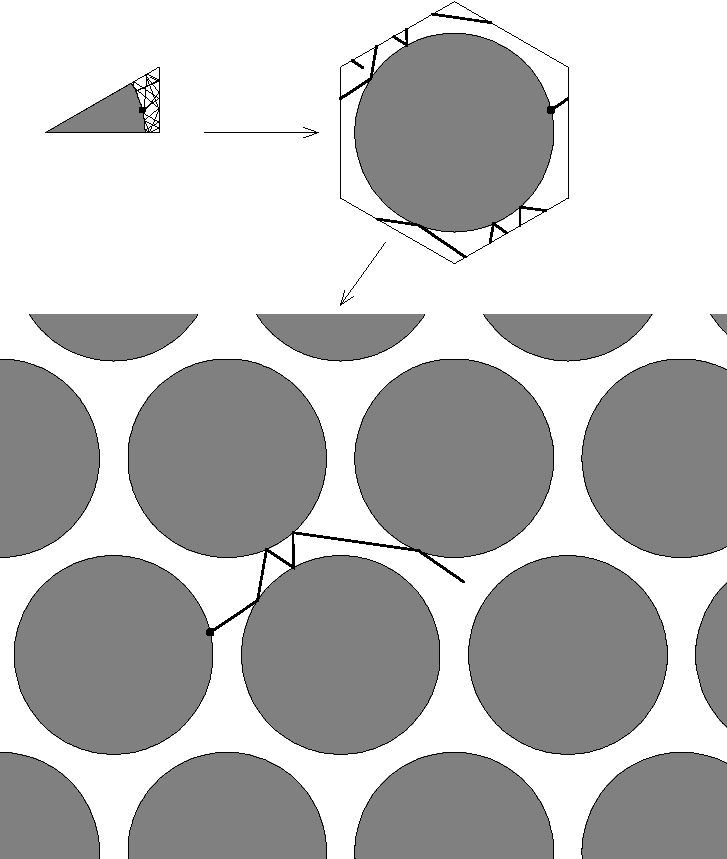
\includegraphics[width=0.45\textwidth]{diffuseSchreiberFig1}
    (b)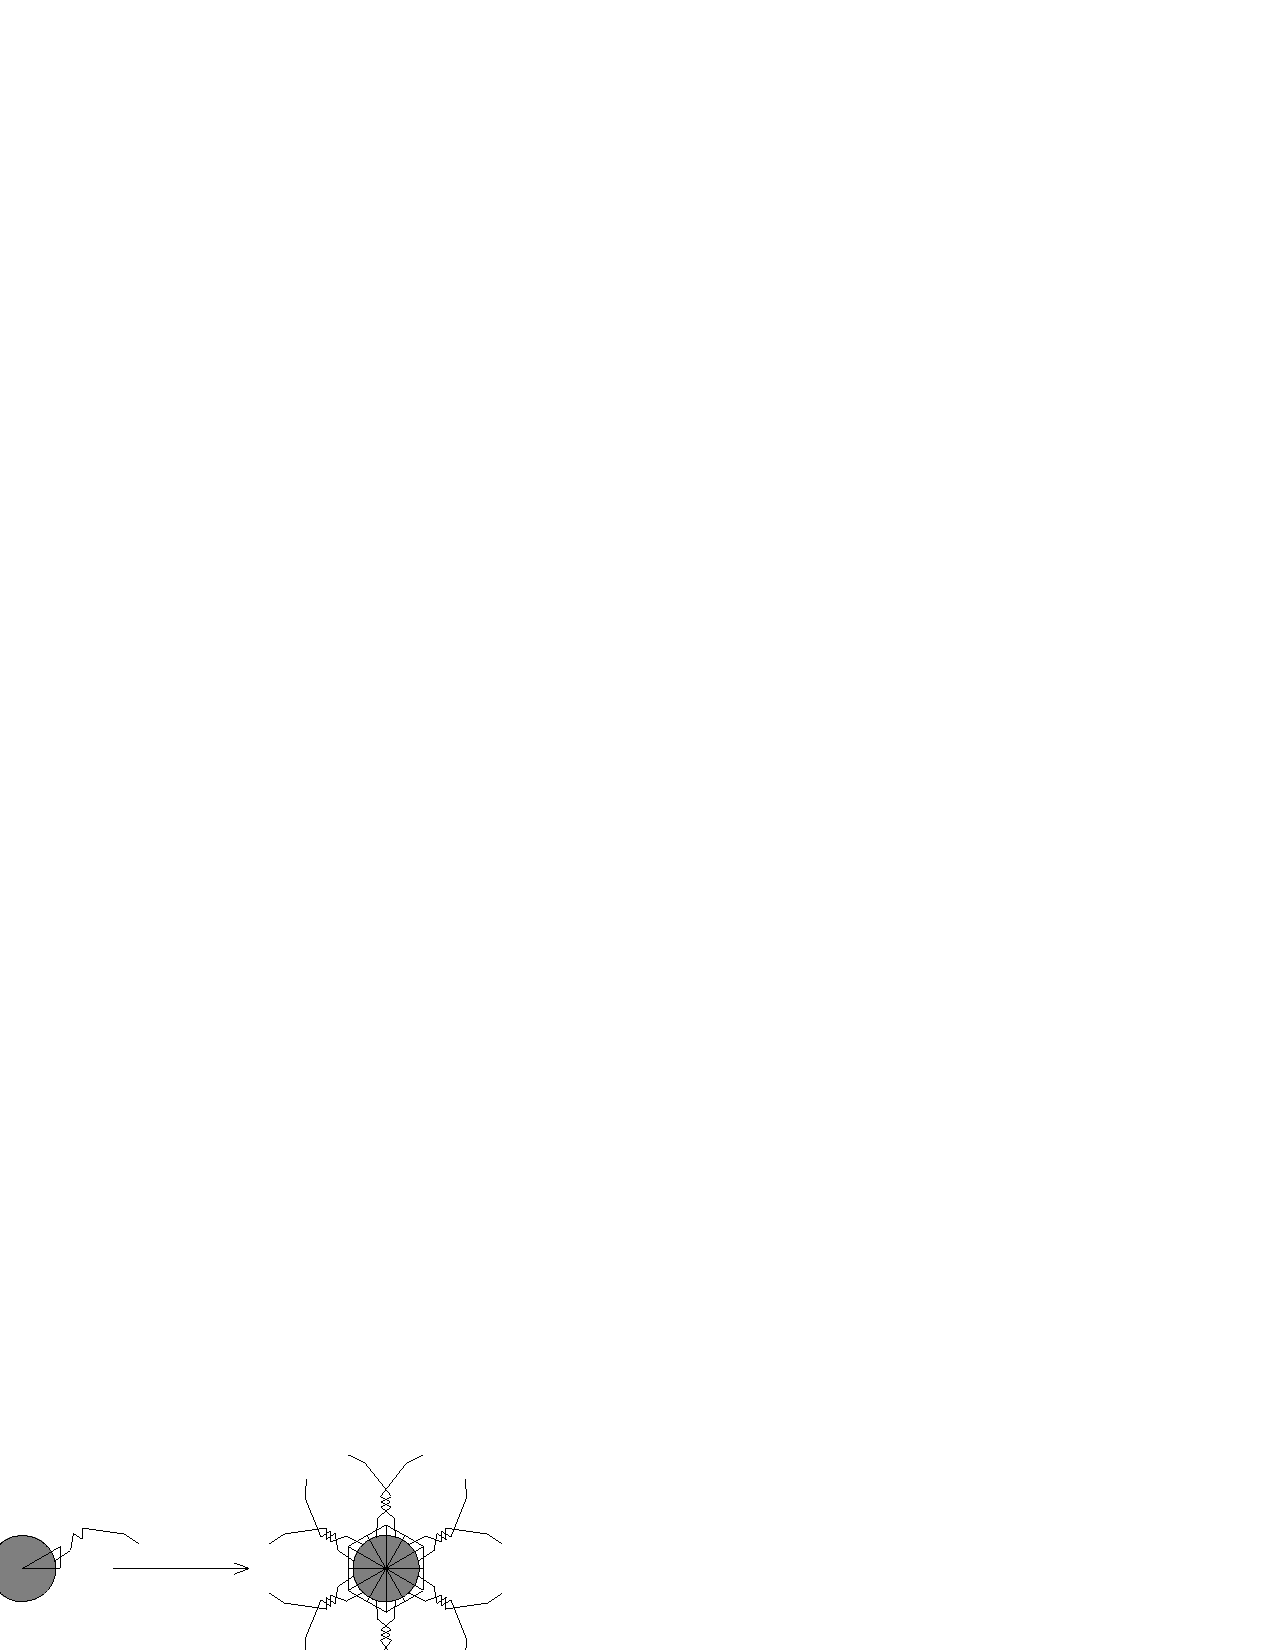
\includegraphics[width=0.45\textwidth]{diffuseSchreiberFig2}
  \end{center}
  \caption[]{\label{fig-schrieberFig12}
  (a) Motion in the fundamental domain (top left), elementary cell (top
      right) and  in full space (bottom).
  (b) An (unwrapped) trajectory (in full  space) and its 12 copies after
      applying point group actions to it.
  }
\end{figure}

%\begin{figure}[htbp]
%  \begin{center}
%    (a)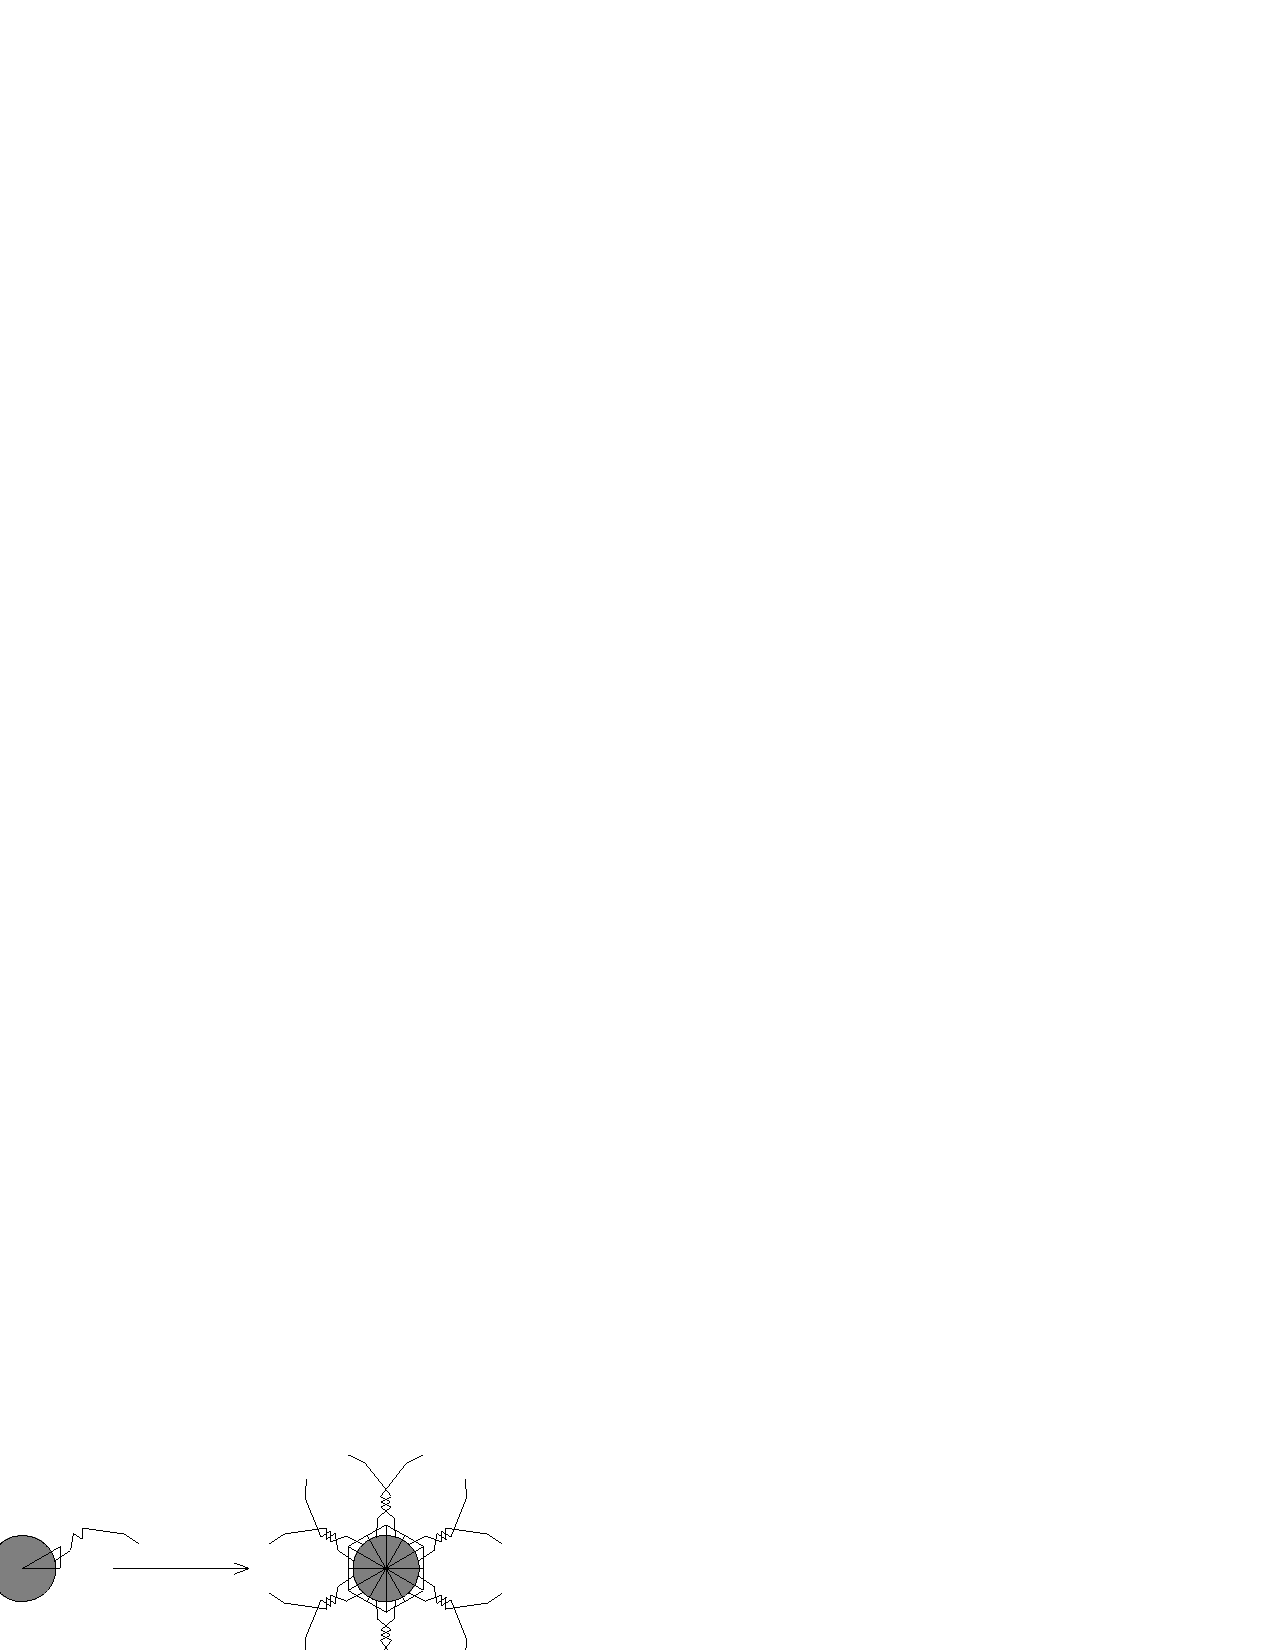
\includegraphics[width=0.45\textwidth]{diffuseSchreiberFig2}
%    (b)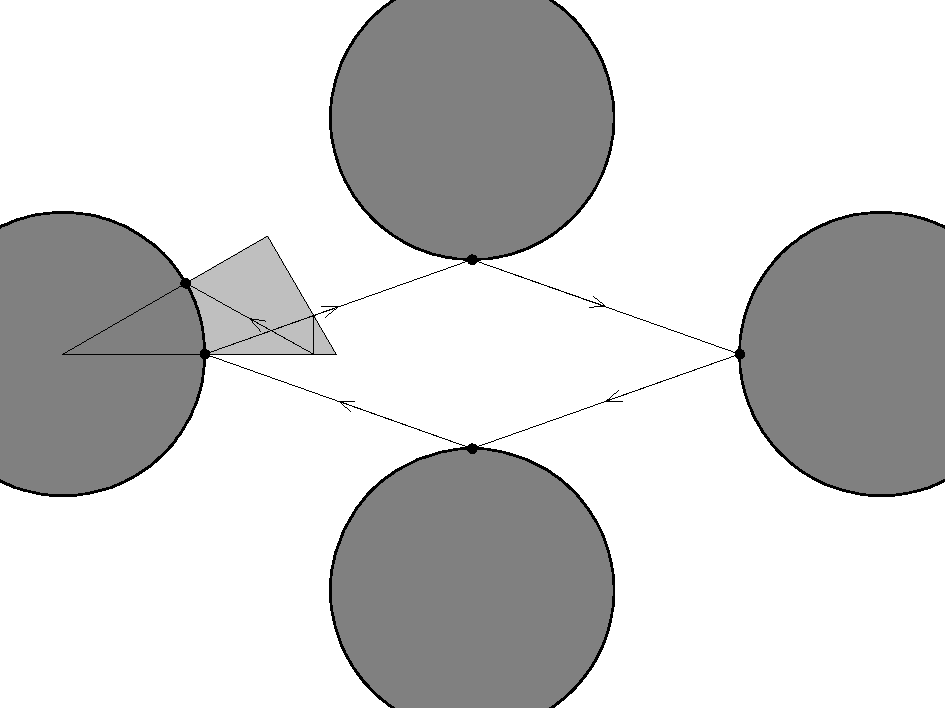
\includegraphics[width=0.45\textwidth]{diffuseSchreiberFig3}
%  \end{center}
%  \caption[]{ \label{fig:schrieberFig23} (a) An (unwrapped) trajectory (in full
%  space) and its 12 copies after applying point group actions to it. (b)
%  Multiplicity of periodic orbits in fundamental domain.}
%\end{figure}

When the scattering array has further discrete symmetries, such as
reflection symmetry, each elementary cell may be built from a {\em
fundamental domain} ${\widetilde \pS}$ by the action of a discrete (not
necessarily abelian) group $G$. The quantity $\tx(t)\,=\,\tflow{t}{\tx}$
denotes the flow in the fundamental domain ${\widetilde \pS}$;
$\tflow{t}{\tx}$ is related to$\flow{}{\tx}$ by a discrete symmetry $g
\in G$ which maps $\tx(t)\in{\widetilde \pS}$ to ${x}(t) \in {\pS}$. The
full $\hM \rightarrow {\widetilde\pS}$ reduction is complicated by the
non-abelian nature of $G$, and will be illustrated in this section in
detail.

\subsection{How point group changes translation}

In the fundamental domain, one has to realize a few facts before
proceeding to the cycle expansion derivation. A point $x$ in the
elementary cell can be uniquely identified by its ``mirror image'' in the
fundamental domain:
\[ %beq
x=g\circ\tx,
\] %eeq
given a group action $g\in G$ the discrete symmetry group. In the
triangular periodic Lorentz gas the underlying point group is $C_{6v}$
(isomorphic to $D_6$), and the hexagonal elementary cell is partitioned
into 12 identical triangular domains. We have to appreciate that the flow
$\hat{\phi}^t$ is G-equivariant under the lattice group symmetry, and
proceed with the argument that the displacement in full space is also
equivariant under the point group symmetry (which is a subset of the
lattice group):
\[ %beq
\hn_t(x)\equiv\hn_t(g\circ\tx)= g\circ\hn_t(\tx).
\] %eeq

We can apply this fact to the displacement associated with a prime
periodic orbit $\tp$ restricted in the fundamental domain.
Let$\tp\equiv\{\tx_0,\tx_1,\ldots,\tx_{N_\tp}\}$, with topological length
$N_\tp$and $\tx_i$ the bouncing points on the orbit. For each flight
(e.g. from $\tx_i$to $\tx_{i+1}$) we denote the associated displacement
in full space $\hn(\tx_i,e)$. However, one has to be careful when adding
the individual displacements together when moving along a fundamental
domain orbit. Unlike in elementary cell, the fundamental domain point
$\tx_i$ does not distinguish in which triangular piece it is. Instead, we
assign a point group element$g_\tp(\tx_{i+1},\tx_{i})$ to keep track of
changes in absolute orientation. We now write the displacement traveled
along the orbit, after finishing a full cycle:
\beq
\hn_{\tp}(\tx_{0})=\sum_{i=0}^{N_\tp-1}\hn(\tx_{i},g_{\tp,\tx_0}(\tx_{i}))=\sum_{i=0}^{N_\tp-1}g_{\tp,\tx_{0}}(\tx_{i})\circ\hn(\tx_{i},e),
\eeq
where $g_{\tp,\tx_{0}}(\tx_i)=\prod_0^{j-1} g_\tp(\tx_{j+1},\tx_{j})$ is
the accumulated orientation changes along the orbit when starting from
$\tx_{0}$.The displacement now has its dependence on the starting point
we choose. We denote the total group action for the orbit

\bea
h_{\tp}(\tx_i)&\equiv& g_\tp(\tx_{i},\tx_{i-1})\circ\ldots\circ
g_\tp(\tx_{0},\tx_{N_\tp-1})\nonumber\\
&& \circ g_\tp(\tx_{N_\tp-1},\tx_{N_\tp-2})\circ \ldots\circ
g_\tp(\tx_{i+1},\tx_{i}),
\eea
which one can immediately see the connection
$\flow{t_\tp}{\tx_i}=h_{\tp}(\tx_i)\tflow{t_\tp}{\tx_i}$.
Although the group action $h_{\tp}(\tx_i)$ depends on the initial points
on the orbit, it is a property of the orbit's symmetry, and subsequently
all $h_{\tp}(\tx_i), \tx_i\in\tp$ belong to the \emph{same} subgroup of
$G$.

We define the quantity:
\beq
\hat{L}_{\tp}^{r}(\tx_i)\equiv
(e+\hp^{1}(\tx_i)+\cdots+\hp^{r-1}(\tx_i))\cdot\hn_{\tp}(\tx_i),
\label{eq-fdDisplacement}
\eeq
to be the displacement traveled along the orbit $r$ times, starting from
$\tx_i$.  Though one may not appreciate immediately,
\refeq{eq-fdDisplacement} takes care of the rotational symmetry that does
not commute with translation, and we will show that it gives the proper
displacement needed for computing diffusion coefficient in the
fundamental domain.


\subsection{Gymnastics of equations}

We properly treat the discrete symmetry by projecting the trace of\evOper
\refeq{eq-eOper} to the group's subspace:
 \bea
\tr{\cal L}^t &=& \sum_{\alpha \in\II_G} \tr{\cal L}_{\alpha}^t\nonumber\\
\tr{\cal L}_{\alpha}^{t} &=& \frac{d_\alpha}{|G|}\sum_{\sigma \in
  G}\sum_{h\in G}\chi_\alpha(h)\int_{\t {\cal M}} d\tx \delta (h\tx -
\flow{t}{\tx})e^{\beta\cdot\sigma\cdot\hn^t(\tx)}.\nonumber\\
\label{eq-traceSum}
\eea

The $\delta$-function part $\delta (h\tx - \flow{t}{\tx})$ in the integral
selects the fundamental domain periodic points that satisfy the group
condition $h\equiv h^r_{\tp}(\tx_i)$. The displacement traveled starting
from each of those points and along the orbit $r$ times takes the form
already computed in\refeq{eq-fdDisplacement}. The rest is straight
forward gymnastics of algebra,which yields the dynamical zeta function
for the $\alpha$ irreducible representation:
\begin{widetext}
 \beq
\frac{1}{\zeta_{\alpha}(\beta,s,z)}
=\exp\left(-\frac{d_\alpha}{|G|}\sum_{\sigma\in G}\sum_{\tp}
    \frac{1}{N_{\tp}}\sum_{\tx_{i}\in\tp}\sum_{r=1}^{\infty}
    \frac{t_{\tp}^{r}}{r}
    \chi_{\alpha}(\hp^{r}(\tx_i))e^{\beta\cdot\sigma\cdot\hat{L}_{\tp}(r,\tx_i)}
    \right),
\label{eq-fdZeta}
\eeq
\end{widetext}

where
\[
  t_{\tp}\equiv
\frac{z^{N_{\tp}}e^{-sT_{\tp}}}{|\ExpaEig_\tp|}
\,,
\]
is the weight associated to the orbit. Equation \refeq{eq-fdZeta}
differs from its counterpart in elementary cell, but can be reduced to if
the symmetry group contains only $e$.

We are interested in the one dimensional, symmetric trivial
representation with$ d_\alpha = 1 $ and all $ \chi(h) = 1 $; there by we
drop the subscript $\alpha $ in the following calculation. Partial
derivative with respect to$\beta$ gives:
\begin{widetext}
\bea
\frac{\partial^{2}}{\partial\beta^{2}}\frac{1}{\zeta(\beta,s,z)}
&=\frac{1}{\zeta(\beta,s,z)}\left(\left(\frac{1}{|G|} \sum_{\sigma\in G}\sum_{\tp}\sum_{\tx_i\in \tp}\sum_{r=1}^{\infty}\frac{\sigma\cdot \hat{L}_{\tp}^{r}(\tx_i)t_{\tp}^r e^{\beta\cdot\sigma\cdot \hat{L}_{\tp}^{r}(\tx_i)}}{N_{\tp}r}\right)^{2}\right.\nonumber\\
&\left.-\frac{1}{|G|}\sum_{\sigma\in G}\left(\sum_{\tp}\sum_{\tx_i\in
      \tp}\sum_{r=1}^{\infty}\frac{\vert \sigma\cdot
      \hat{L}_{\tp}^{r}(\tx_i)\vert^{2}t_{\tp}^{r}e^{\beta\cdot\sigma\cdot
        \hat{L}_{\tp}^{r}(\tx_i)}}{N_{\tp}r}\right)\right).
        \eea
\end{widetext}
The first term in the formula corresponds to $ \langle\hx\rangle^2 $ and
second to $ \langle\hx^2\rangle $. It is trivial to see that
\beq\sum_{\sigma\in G}\frac{\sigma\cdot
  \hat{L}_{\tp}^r(\tx_i)t_{\tp}^r e^{\beta\cdot\sigma\cdot
  \hat{L}_{\tp}(r,\tx_i)}}{N_{\tp}r} \equiv 0,
\eeq
because of the summation over the discrete group $G$. Thus the calculated
mean drift is zero, consistent with the symmetry of the system. Observing
that the length$\vert \sigma\cdot \hat{L}_{\tp}^{r}(\tx_i) \vert$ does
not change under rotation, we write
\bea
\langle\hx^2\rangle &=& \left.\frac{1}{\zeta(\beta,s,z)}\sum_{\tp}\sum_{r=1}^{\infty}\frac{t_{\tp}^{r}}{r}\sum_{\tx_i\in \tp}\frac{\vert\hat{L}_{\tp}^{r}(\tx_i)\vert^{2}}{N_{\tp}}\right\vert_{\beta=0,s=0, z=1} \nonumber\\
&=& \left.\prod_{\tp}\left(1-\frac{z^{N_{\tp}}}{\vert\ExpaEig_\tp\vert
    }\right)\sum_{\tp}\sum_{r=1}^{\infty}\left(\frac{z^{N_{\tp}}}{\vert\ExpaEig_\tp\vert
    }\right)^r\frac{\vert\hat{L}_{\tp}^{r}\vert^2}{r}\right\vert_{z=1}
\label{eq-meanSquareDisp}
\eea with $\hat{L}_{\tp}^{r}\equiv\sum_{\tx_i\in
  \tp}\frac{\vert\hat{L}_{\tp}^{r}(\tx_i)\vert^{2}}{N_{\tp}}$ the
average square displacement in full space when traveling along a fundamental domain $r$ times. Formula \refeq{eq-meanSquareDisp} is an infinite polynomial in the auxiliary variable $z$, and should be truncated to the topological length of the longest periodic orbits find in calculation.

\subsection{Grammar of fundamental domain cycle}

\begin{figure}[htbp]
  \begin{center}
    (a) 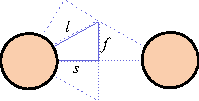
\includegraphics[width=0.35\textwidth]{diffuse7diskFundDflips}
    (b) 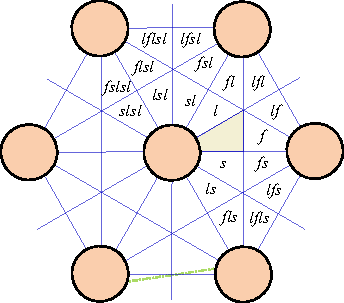
\includegraphics[width=0.35\textwidth]{diffuse7diskFundDtiles}
  \end{center}
  \caption{\label{fig-7diskFundDflips}
  (a) The three generators of tiling of the  plane by a fundamental
  domain: two generators of \Dn{12} tiling, reflection  $s$ across the
  short disk-disk separation, reflection $\ell$ across the long
  disk-disk separation; and a translation generator $f$ that pivots
  (`flips') a  disk center to disk center by flip across the symmetry
  line normal to the short disk-disk separation.
  (b) Tiling of the 7-disk by copies of the fundamental domain, labeled
  by a (not unique) sequence of the three generators  $\{s,\ell,f\}$,
  chosen so that each sequence contain one and only on  disk-to-disk
  pivot $f$.
  }
\end{figure}
    \TZ{2015-10-19}
    {I do not really use the three generators to compute the fundamental
    domain cycles, instead I use the idea of topological distinct flights
    (\reffig{fig-fdflights}). We have yet to discuss the equivalence
    between the 3-generators and topological distinct flight in the two
    figures. }

\begin{figure}[htbp]
  (a)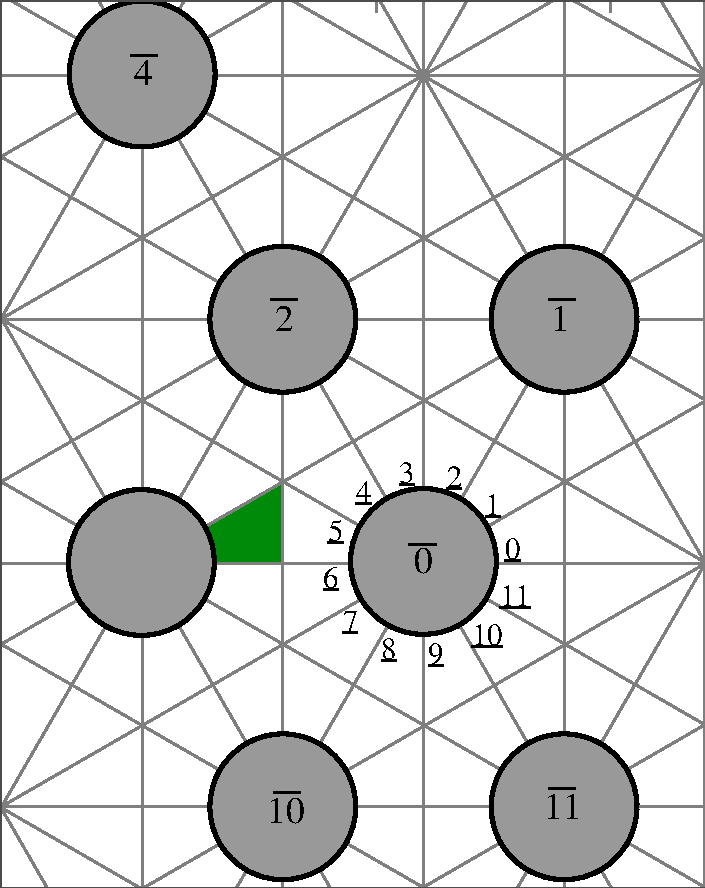
\includegraphics[width=0.35\textwidth]{diffuseFDSymbolIllustration}
  (b)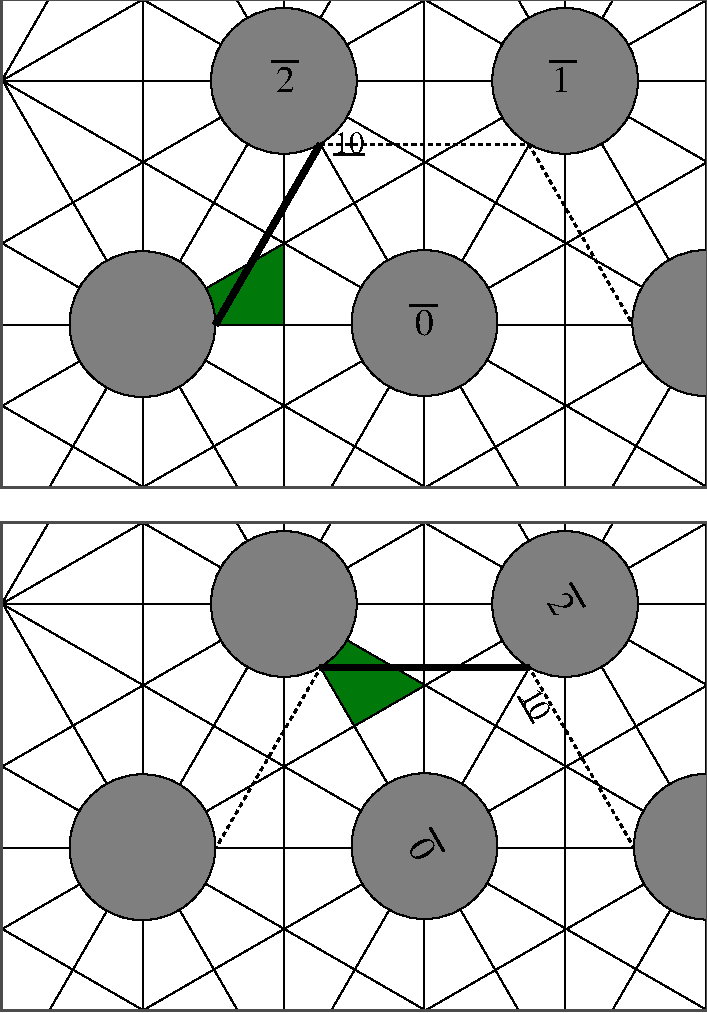
\includegraphics[width=0.35\textwidth]{diffuseFDSymbolOrbits}
  \caption{\label{fig-fdflights}
  Fundamental domain symbolic dynamics.
  (a) With  imposed finite horizon and starting on the edge of a disk in
  fundamental  domain (the green filled region), there are at most 6
  disks can be reached  without collision (disk
  $\overline{0},\overline{1},\overline{2},\overline{4},\overline{10}$ and
  $\overline{11}$). Similar to how elementary cell symbolic dynamics are
  created, we label the 12 triangular pieces of a disk in a counter
  clock-wise  manner, from $\underline{0}$ to $\underline{11}$. The
  combination of a disk  label and a triangular piece label
  $\{\overline{i},\underline{j}\}$ uniquely  identifies a topologically
  distinct flight.
  (b) The fundamental domain fixed point
  $\{\overline{2},\underline{10}\}$, which corresponds to a periodic
  orbit of length 6 in elementary cell ($\cycle{0246810}$), is unwrapped
  in   global space. After each collision we re-label the disks and
  triangular   partitions according to their relative positions to the
  ``new'' fundamental   domain. In the figure labels are also rotated
  according to the point   group actions.
  }
\end{figure}



In the international crystallographic notation, the hexagonal lattice is
called $p6mm$, with point group $6mm$, where prefix $p$ indicates that
the unit cell is primitive (not centered),
\beq
\Group = \{
e, C_6^+, C_6^-, C_3^+, C_3^-, C_2,
\sigma_{d1}, \sigma_{d2}, \sigma_{d3},
\sigma_{v1},\sigma_{v2}, \sigma_{v3}
\}
\,,
\eeq
with $s=\sigma_{d}$ the reflection across the short disk-disk separation,
and $\ell=\sigma_{v}$ reflection across the long disk-disk separation
generators of \Dn{12}. The entire space group $p6mm$is then generated by
adding a disk-to-disk generator $f$ that pivots a disk center to another
by flip across the symmetry line normal to the short disk-disk
separation, \reffig{fig-7diskFundDflips}a. We find it convenient to
define $C$ as the generator of cyclic rotations by $\pi/3$,
\beq
\ell s = C_6^- = C
\,,\quad
C^6 = e
\,;\qquad
s \ell =  C_6^+
\,,\qquad
s  =  C_6^+ \ell
\,.
\eeq
    \TZ{2015-10-22}
    {The idea is that the topological periodic orbit in the fundamental
    domain is not sensitive to the order of flips. When $w$ increases,
    one might notice that a single flight along the orbit changes from
    $sf$ to $fs$. However, the relative position between the start and
    end triangular cells are always the same.}
A free flight between two disks in the full space may then be wrapped
into fundamental domain, according to the sequence cell edges
$\{s,\ell,f\}$ it passed. For example, there are different paths when
jump to disk $0$: it can be as simple as a single pivot about $f$, or can
be more complex such like $\ell f s$ that involves multiple flips,
~\reffig{fig-7diskFundDflips} b. Although we can associate each free
flight with a chain of the generators, some of the combinations are
equivalent. The short jump $sf$ is topologically equivalent to $fs$, in
the sense that the particle ends up in the same copy of fundamental
domain before next collision.

Our task is to generate all distinct itineraries from $\{s,\ell,f\}$. One
can immediately realize a partial list of the equivalence relations:
\bea
f s &=& s f
\,,\nonumber\\
f \ell f&=&\ell f \ell
\,.
\eea
All longer equivalence relations in ~\reffig{fig-7diskFundDflips} can be
reduced to the above primitive ones:
\bea
f s \ell &=& s f \ell\,,\nonumber\\
\ell f\ell s &=& f \ell s f\,.
\eea

There are also some pruning rules to keep in mind. Because a free flight
cannot cross the same border twice, sequences including $\ell\ell,ff,ss$
are forbidden. $C^3$ (and all higher orders) is also pruned as the
particle cannot cross the center hard disk; nor swirl around it.

While the string description of flight is mathematically rigorous and
accurate, it is practically hard to be encoded into programs for
computing the orbits, because the number of equivalent strings increases
exponentially when the length (of a single string) increases. However,
there is a more physically intuitive way to organize the type of flight,
by means of ``topological flight'', \reffig{fig-fdflights} (a). In this
representation, a equivalence relation like $sf\equiv fs$ can be uniquely
identified by a combination of a disk number and a partition number
$\{\overline{0},\underline{6}\}$. Longer flight such like $\ell f \ell s
\ell f \equiv  f \ell f s \ell f \equiv f \ell s f \ell f \equiv f \ell s
\ell f \ell$ that cross many boundaries now yields a very simple symbol
pair $\{\overline{1},\underline{5}\}$.

The topological flight leads to a straight forward numerical scheme to
find cycles. The disk number fixes the two ends of the free flight while
the partition number limits the range of angles on the disk. Similar to
searching cycles in elementary cell, we now have a constrained version of
numerical minimization problem which can be solved using standard
non-linear optimization approach.
 \TZ{2015-11-02}
    {I have not yet talked about the pruning rule in detail here; it is
    more complicated bases on the reflection angle}

\subsection{Diffusion in the fundamental domain}
\begin{table}[htbp]
\hfill
\TZ{2015-10-19}{Do we need this many digits in the table?}
\begin{tabular}{|r|r|r|l|l|}
\hline
$\period{p}$ & \# cycles & $\zeta$(0,0) & $\lambda$ & D \\ \hline\hline
1      & 5      & -0.2169759 & 1.39193 & 0.37795 \\
2      & 10     & -0.0248233 & 1.74541 & 0.23118\\
3      & 33     & -0.0221962 & 1.72235 & 0.25257\\
4      & 108    & -0.0002192 & 1.74450 & 0.24165\\
5      & 373    &  0.0023463 & 1.76079 & 0.24468\\
6      & 1378   &  0.0096330 & 1.75610 & 0.24068\\ \hline\hline
\multicolumn{3}{|l|}{numerical experiment}
                           & 1.760 & 0.25
\\ \hline
\end{tabular}

\caption{\label{TCELL2}
  Results for $w$=0.3. Calculation in FD. Gaspard 1992
  note: ``My numerical estimate for the Lyapunov exponent when $w=0.3$ is
  $\lambda = 1.760 \pm 0.002$, which supports the result of this table.''
}
\end{table}

\begin{figure}[htbp]
  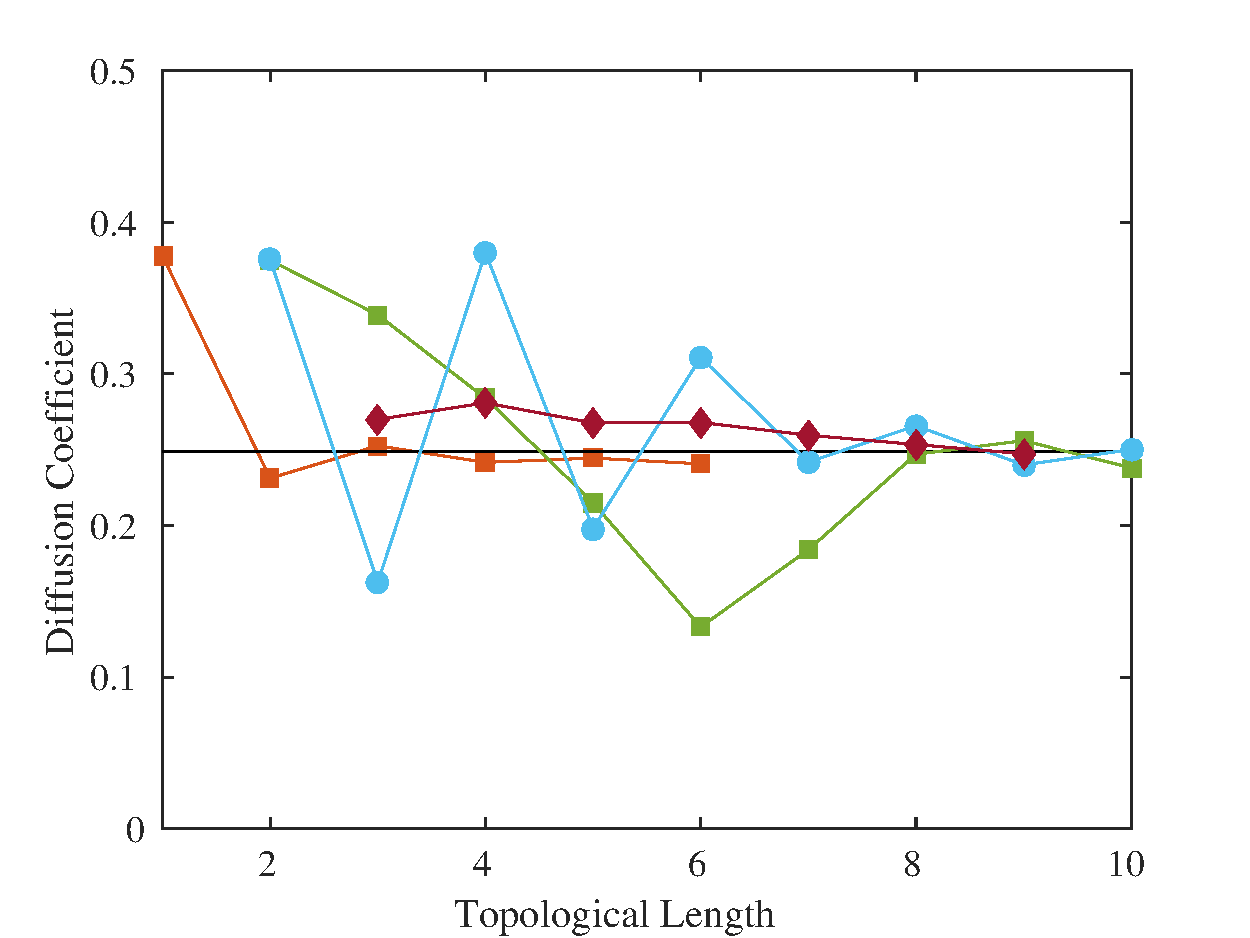
\includegraphics[width=0.45\textwidth]{diffuseCycleExpansionResults}
  \caption[]{\label{fig-convergence}
  The convergence of diffusion coefficients  calculated using cycle
  expansion in elementary cell (green squares),  fundamental
  domain(orange squares). We  also show the convergence of ``periodic
  orbit expansion'' method, with and  without Shanks transformation
  (circles and diamonds) discussed in  \refref{Morriss1994}. Here $w = 0.3$.
  }
\end{figure}

\begin{figure}
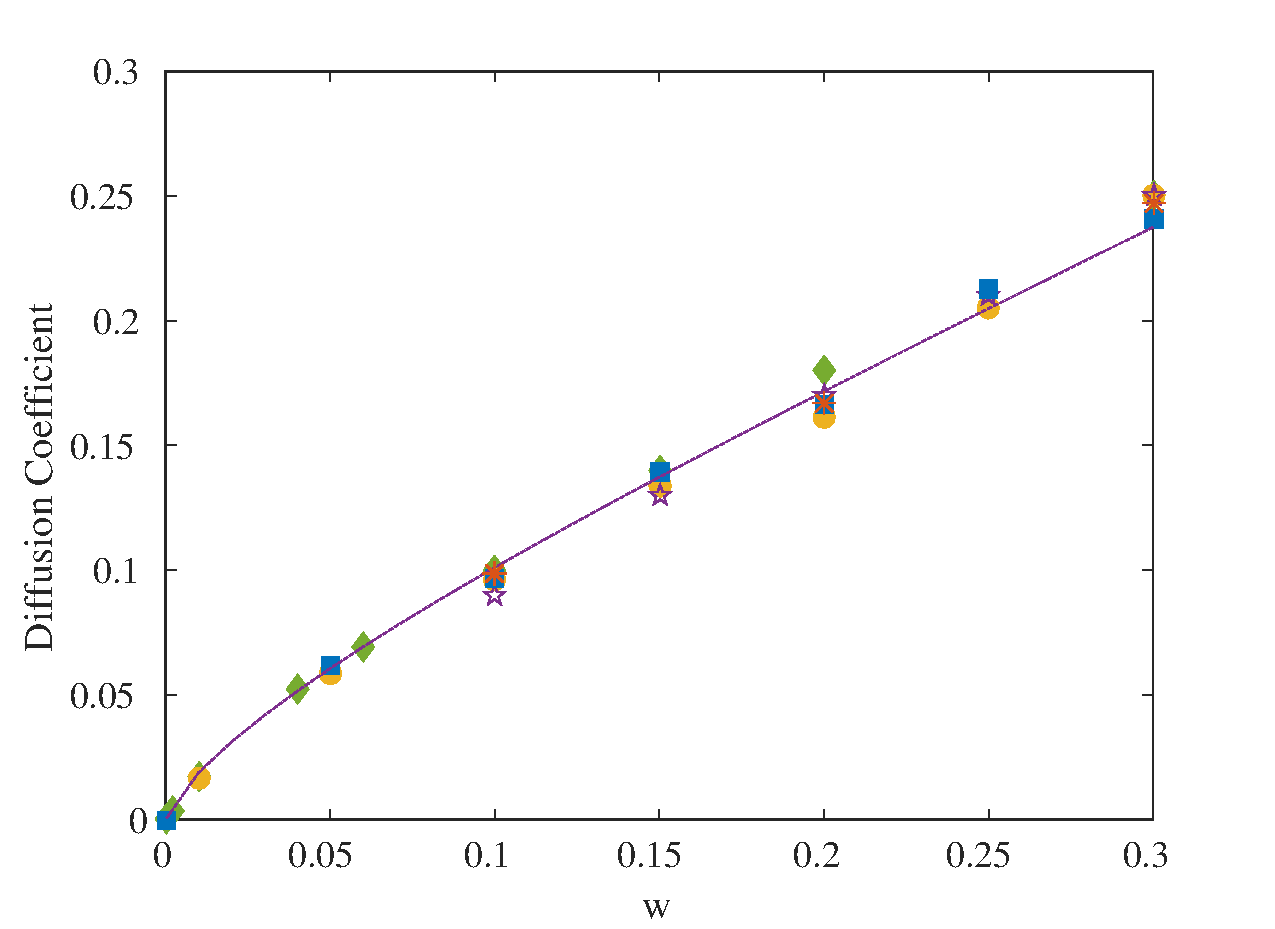
\includegraphics[width=0.45\textwidth]{diffuseDiffCoefPlot}
  \caption[]{\label{fig-results} Diffusion coefficients as a function $w$.  Figure generated using data from various resources. Diamonds are results from  Green-Kubo numerical experiments\rf{MacZwa83}; stars\rf{BaEvCo93} and  circles\rf{GasBar95} are calculated from escape rate; and triangles are  given by Hausdorff fractal dimension calculation\rf{GasBar95}; dashed line  is a statistical approximation\rf{Angstmann20121819}}.
\end{figure}

       \TZ{2015-10-19}{Any comment on caption of \reffig{fig-convergence}?}
Compared with various methods, the symmetry reduced cycle expansion
method converges the fastest, table \ref{TCELL2} and
\reffig{fig-convergence}. Diffusion coefficient computed from $\sim2000$
fundamental domain cycles of topological length up to 6 gives two
significant digits, while the elementary cell calculation needs over
$\sim 10000$ cycles in order to converge. In other words, the fundamental
domain cycles suggests a better and denser partition of the phase space.
    \TZ{2015-10-19}{Talk about other two methods}.

To further test \refeq{eq-meanSquareDisp}, we compute the diffusion
coefficient for $w/r = 0.05, 0.10, 0.15, 0.20, 0.25, 0.30$, and compare
the results with existing numerical experiments and a recent statistical
estimation, \reffig{fig-results}. In Green-Kubol velocity
auto-correlation method the  diffusion coefficient can be extrapolated to
the accurate reference value $0.250$ (at $w/r=0.30$), using ensembles of
$10^6\sim10^7$ gas particles flying for long time $T>20$ (and the number
of bounces is greater than this)\rf{MacZwa83}. On the other hand, while
statistical approach yields a smooth analytical
formula\rf{Angstmann20121819}, the diffusion property is fundamentally
never a smooth, monotonically increasing function of $w$
    \TZ{2015-11-02}
    {what is that 1D diffusion reference that shows the anywhere
    continuous, nowhere smooth curve?}
Again, the effectiveness (yet correctness) of the cycle expansion is
proved by those comparison.

\section{Conclusion}

 \TZ{2015-11-02}{What else do we put here?}
% Specify following sections are appendices. Use \appendix* if there
% only one appendix.
%\appendix
%\section{}

\begin{acknowledgments}
We are grateful to Pavel M. Svetlichnyy for many fruitful discussions in
the early stages of this project, and the key suggestion that the plane
can be tiled in terms of three elementary tiling generators.
TZ was supported by NSF grant ???-?????.
PC thanks to the family of late G. Robinson, Jr. and NSF grant
DMS-1211827 for partial financial support.
\end{acknowledgments}

\ifboyscout
% switch to Private
\newpage
    \input ../tingnan/flotsam
% \newpage
\fi


% Choosing a journal automatically selects the correct APS BibTeX style
% file (bst file), so only uncomment the line below if necessary.
% \bibliographystyle{apsrev4-1}
\bibliography{../bibtex/siminos,../bibtex/diffuse}


\end{document}



% If in two-column mode, this environment will change to single-column
% format so that long equations can be displayed. Use sparingly.
% \begin{widetext}
%   put long equation here
% \end{widetext}

% Use the figure* environment if the figure should span
% across the entire page. There is no need to do explicit centering.

% Surround figure environment with turnpage environment for landscape
% figure
% \begin{turnpage}
%   \begin{figure}
%     \includegraphics{}%
%     \caption{\label{}}
%   \end{figure}
% \end{turnpage}

% Here is an example of the general form of a table:
% Insert the column specifiers (l, r, c, d, etc.) in the empty braces of the
% \begin{tabular}{} command.  The ruledtabular enviroment adds doubled
%   rules to table and sets a reasonable default table settings.  Use
%   the table* environment to get a full-width table in two-column Add
%   \usepackage{longtable} and the longtable (or longtable*}
%   environment for nicely formatted long tables. Or use the the [H]
%   placement option to break a long table (with less control than in
%   longtable).
% \begin{table}%[H] add [H] placement to break table across pages
% \caption{\label{}}
% \begin{ruledtabular}
%   \begin{tabular}{}
% Lines of table here ending with \\
% \end{tabular}
% \end{ruledtabular}
% \end{table}

% Surround table environment with turnpage environment for landscape
% table
% \begin{turnpage}
%   \begin{table}
% \caption{\label{}}
% \begin{ruledtabular}
%   \begin{tabular}{}
% \end{tabular}
% \end{ruledtabular}
% \end{table}
% \end{turnpage}
